\chapter{Related Work: $\theta$RARes Model and Its Limitation}\label{issues}

Humans have a remarkable ability to perceive and comprehend one or more languages. But, how do they know what does a sequence of symbols mean? In other words, how do they link a series of words to its meaning? With this research question, Hinaut et al. \cite{xavier:2013:RT} proposed a neuro-inspired model, $\theta$RARes, to process the sentence across time without having to know about the semantics of the words. The model uses the reservoir computing approach namely Echo State Network (ESN) and has been successfully implemented on iCub humanoid robot platform \cite{tra:xavier_hri} for the TRA task. It was the first time when ESN was used for the TRA task. The experiments performed using $\theta$RARes model on the TRA task, showed the results toward modeling of language acquisition in brain \cite{tra:xavier_wermter:2014, xavier:2013:RT}

\section{Overview of $\theta$RARes Model}\label{sec:xavier_model}

\begin{figure}[hbtp]
\centering
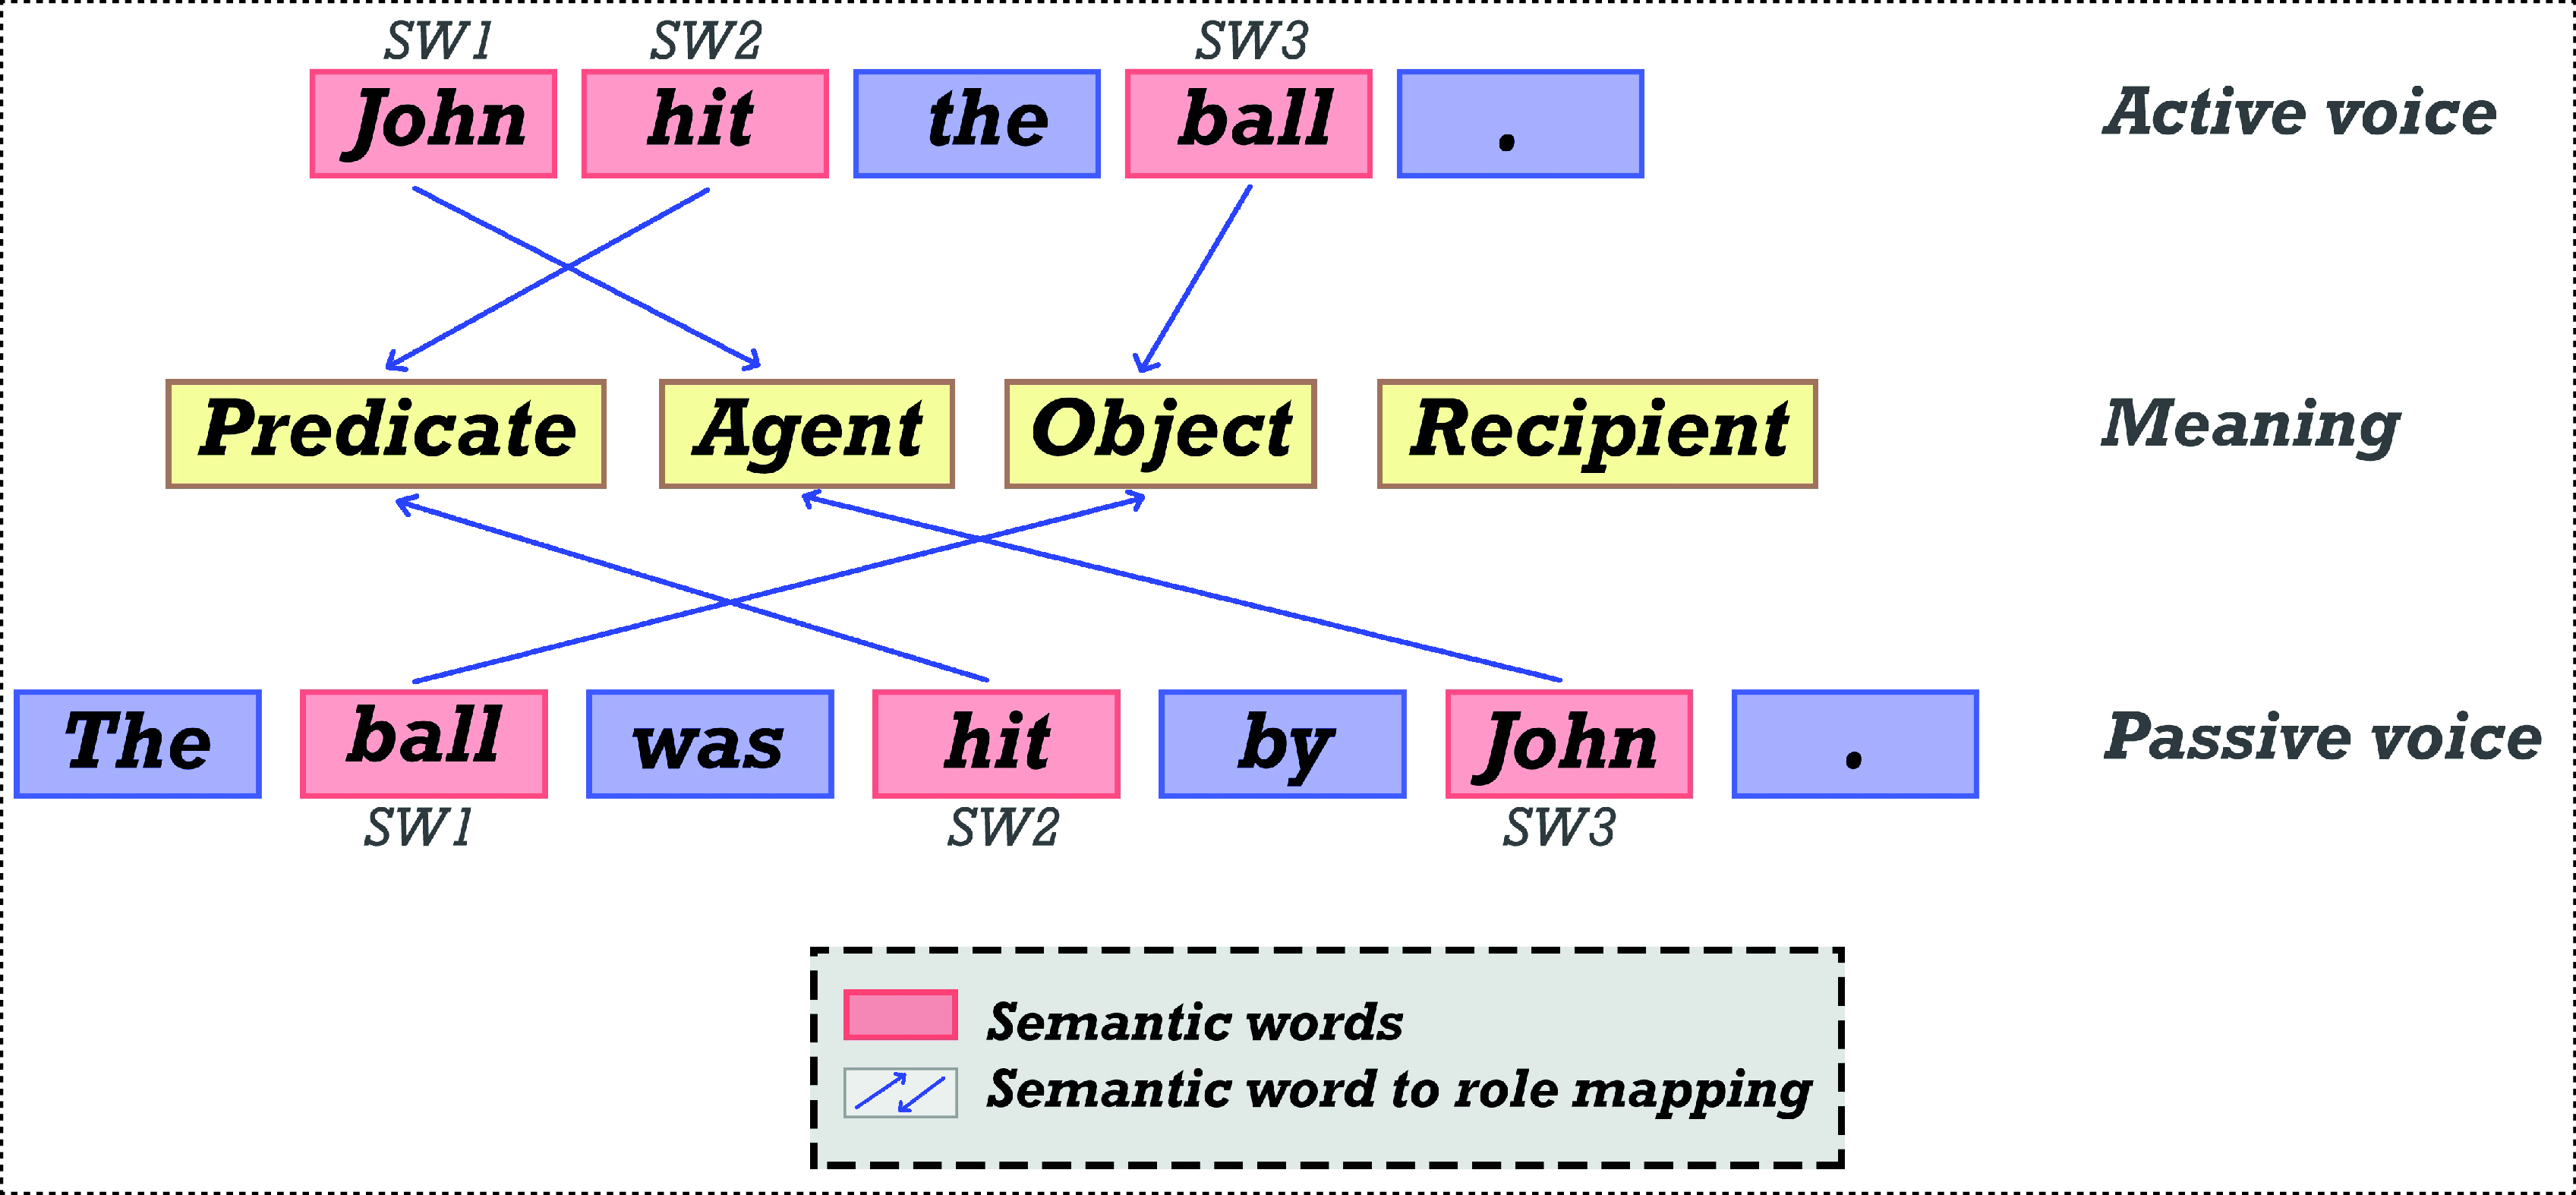
\includegraphics[width=0.8\linewidth]{grammatical_construction}
\caption[Schematic characterization of TRA in grammatical construction.]{\textbf{Schematic characterization of thematic roles in grammatical construction:} {\small The figure shows the mapping (shown with arrows) of semantic words (shown in red) to their thematic roles for an active and passive sentence. The identification of the thematic role of each semantic word in a sentence is defined as the coded meaning of the sentence. Notice that the coded meaning of an active and passive sentence is different, i.e., SW1 is an agent in active sentence whereas the same SW1 is an object in the passive sentence. Despite having the different coded meaning both the sentence share the same sentence meaning, i.e., hit (John, ball). Figure adapted from \cite{xavier:2013:RT}.}} 
\label{fig:tra_gc}
\end{figure}

$\theta$RARes Model is basically an ESN to learn and predict the thematic roles of input sentences. The model is based on the notion of grammatical construction \cite{gc:goldberg:1995} which is defined as the mapping of sentence's surface form (word order) to its meaning \cite{xavier:2013:RT}. Figure \ref{fig:tra_gc} represents the characterization of thematic role assignment for an active and passive sentence in the grammatical construction. To use the notion of grammatical construction, the model utilize the cue competition hypothesis of Bates et al. \cite{tra:bates:1982}, which states that the closed class words (e.g. prepositions, articles, determiners, pronouns, etc.), the order of words and the prosody, encodes the grammatical structure of sentences. Thus in order to map the sentence structure to its meaning, the model does not process the raw sentences but, instead use the abstract grammatical form of the sentences \cite{xavier:2013:RT, tra:dominey:2003}. The abstraction to grammatical form marks each word of a sentence into two kinds of symbols: Functional Words (FWs) and Semantic Words (SWs). Functional words are the closed class words or grammatical words. A closed class is the one which contains a limited number of words, and new words are rarely added to it. In Linguistics, a closed class usually includes determiners, prepositions, articles, pronouns and verb inflections like -ed, -ing or -s, etc. \cite{tra:open_close_class}. Semantic words are the open class words. An open class is the one which accepts new words and usually includes nouns, verbs, adjectives, adverbs, etc. \cite{tra:open_close_class}. 

\begin{figure}[hbtp]
\centering
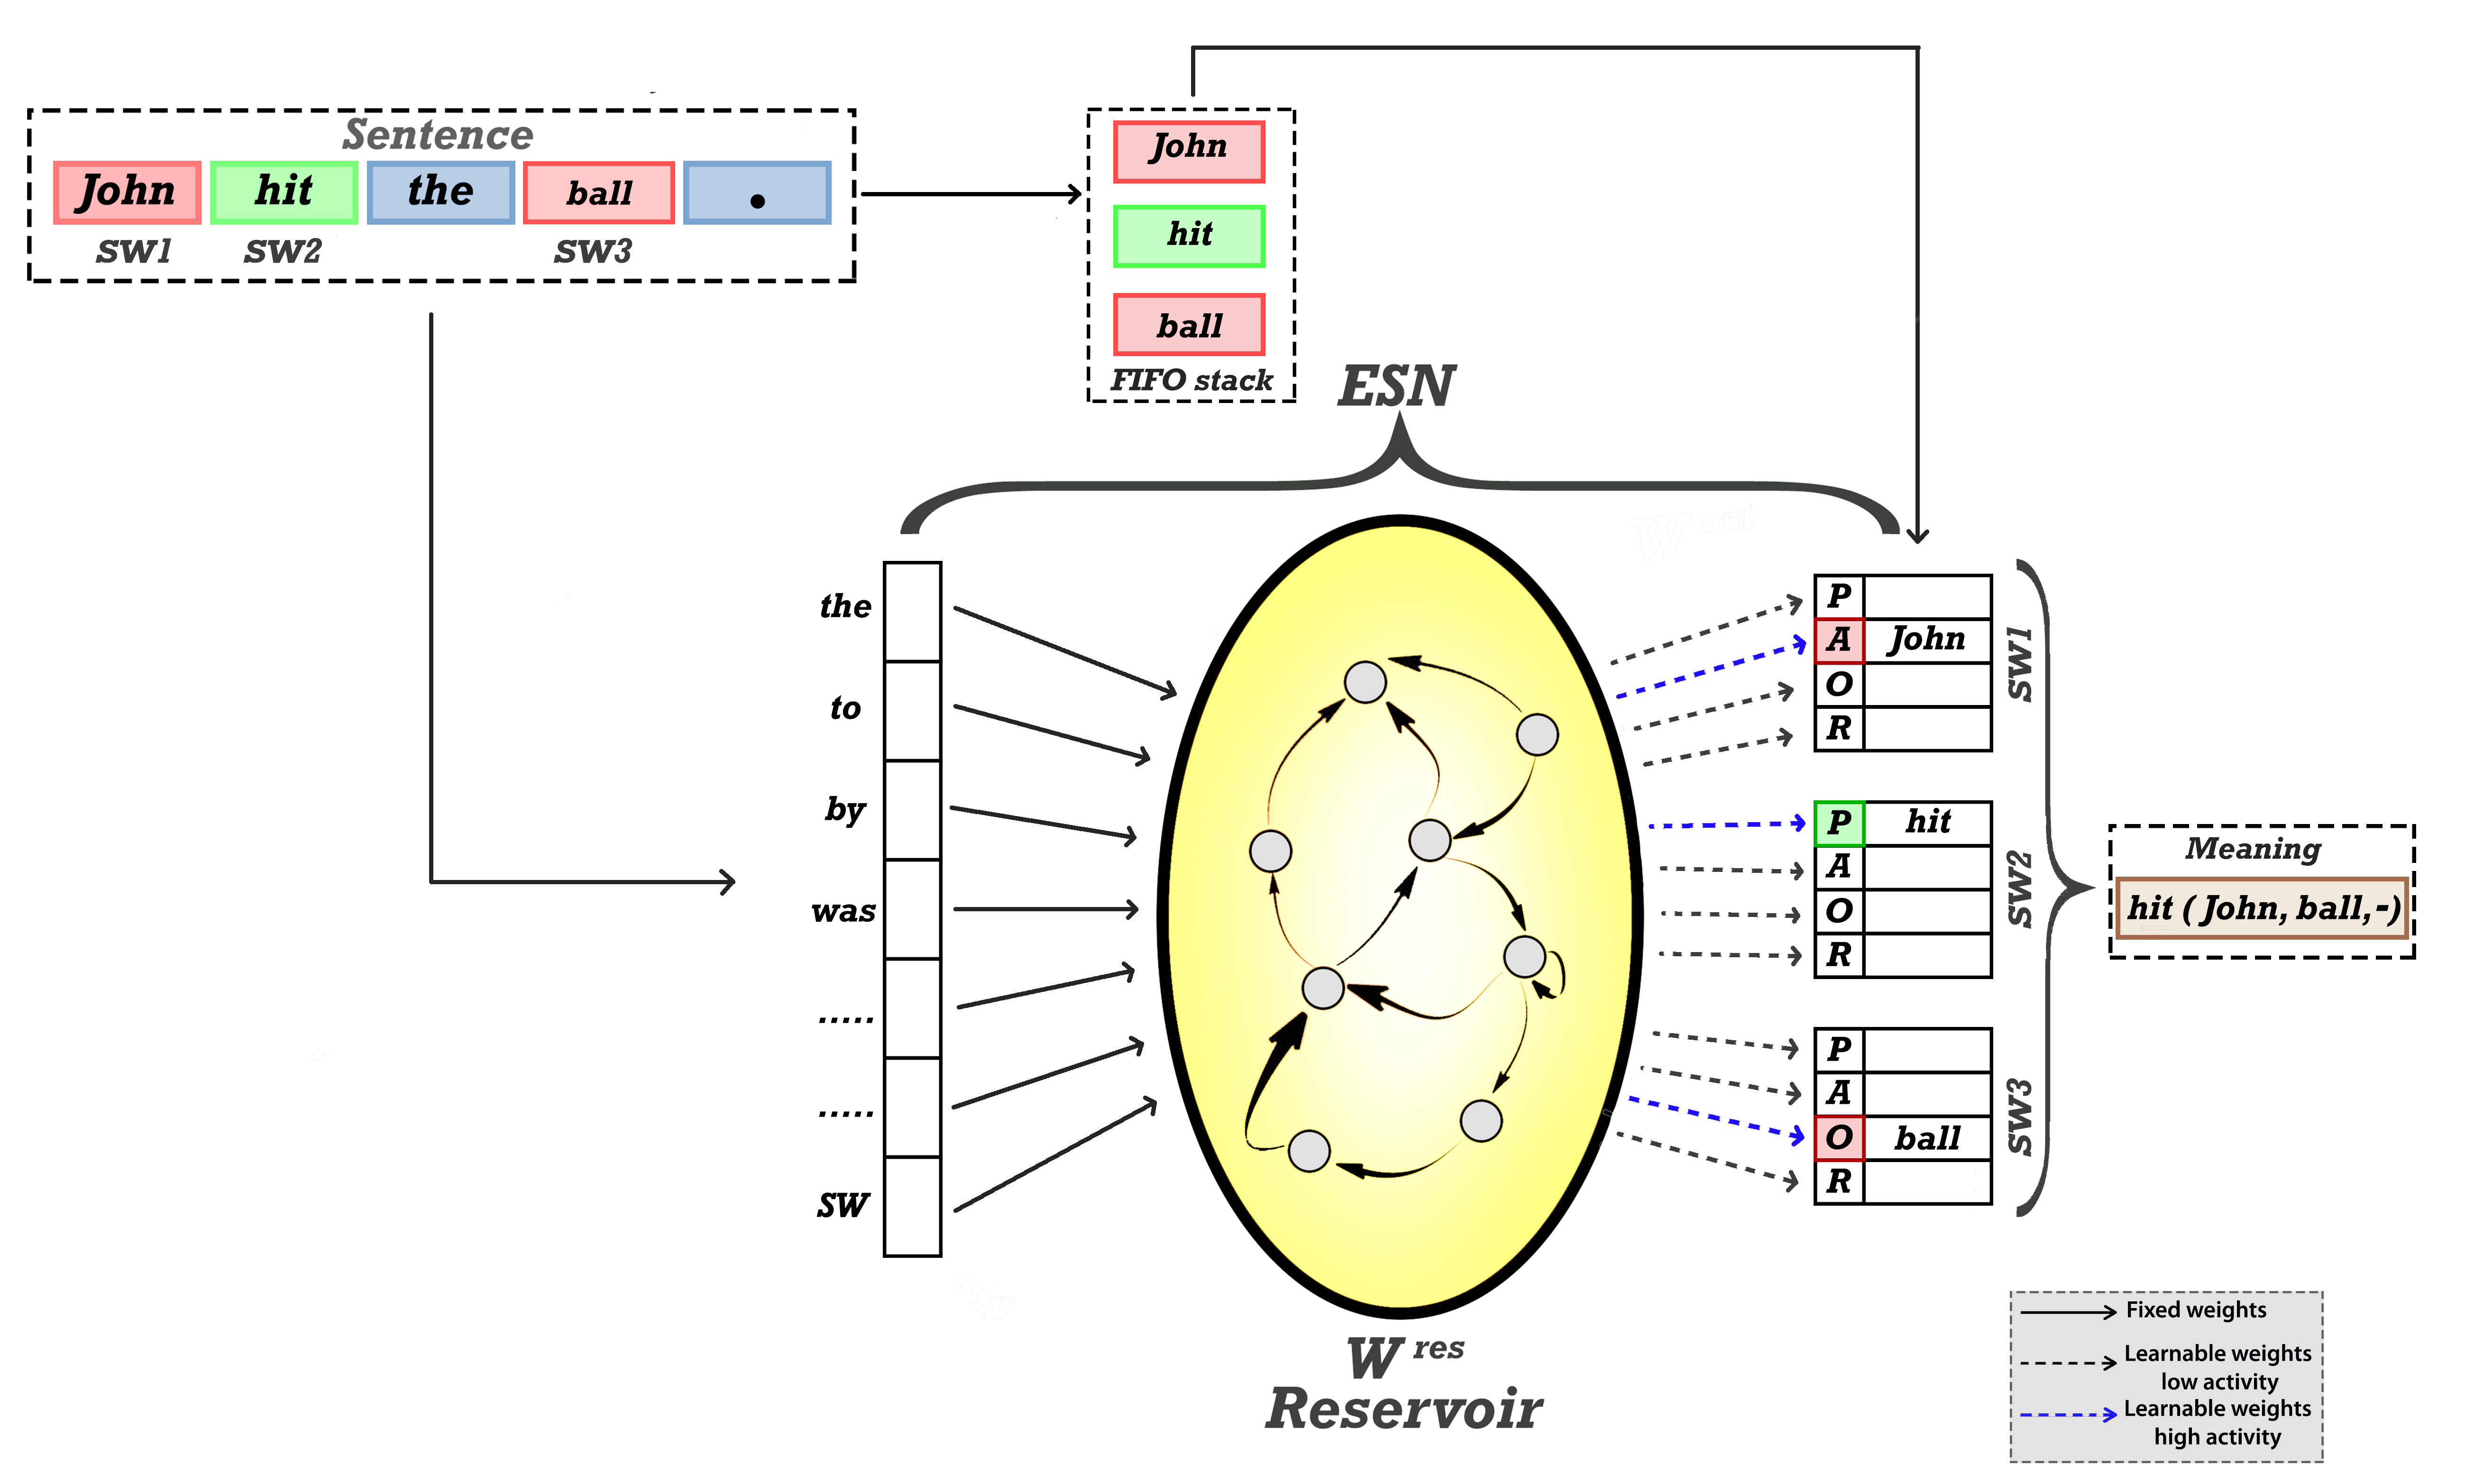
\includegraphics[width=1.0\textwidth]{xavier_model}
\caption[Functional organization of $\theta$RARes language model.]{\textbf{Functional organization of $\theta$RARes language model: }{\small The figure shows the processing of a grammatical construction by $\theta$RARes model. The semantic words (shown in red and green) are separated at the input and stored in a FIFO memory stack. Closed class words and a ``SW" token is input to the model. The model process a sentence, word-by-word, using the localist words vectors as an input. During the training, the coded meaning (i.e. SW1: Agent, SW2: Predicate, SW3: Object) is teacher forced on the output layer, and the readout weights (shown in dotted lines) are learned. While testing the model predicts the coded meaning of the sentence. The meaning of the sentence i.e. hit (John, ball, -) can then be obtained by mapping the coded meaning of a sentence with the semantic words from memory stack. Figure adapted from \cite{xavier:2013:RT}.} }
\label{fig:xavier_model}
\end{figure}

Figure \ref{fig:xavier_model} shows the functional organization of the $\theta$RARes model. A set of closed class words is first defined for the TRA task. Before giving a sentence as an input to ESN, all the semantic words (not in closed class words set) are pushed to a FIFO memory stack (see fig. \ref{fig:xavier_model}) and replaced with a unique token ``SW''. The functional words are left unchanged as the functioning of model completely depends on them \cite{xavier:2013:RT}. This transformation of the sentences to grammatical form by replacing the semantic words with ``SW'' tokens allows the $\theta$RARes model to be trained on a small dataset. This is because one grammatical form can represent several sentences just by replacing the ``SW'' token with different nouns, verbs, etc.

\begin{table}[hbtp]
\centering
\caption[Transformation of a sentence to abstract grammatical form and encoding it using localist word vectors.]{Transformation of a sentence to abstract grammatical form and encoding it using localist word vectors.}
\begin{tabular}{|l|l|l|l|l|l|}
\hline
\multicolumn{1}{|c|}{\multirow{2}{*}{\textbf{Original words}}} & \multicolumn{1}{c|}{\multirow{2}{*}{\textbf{Grammatical form}}} & \multicolumn{4}{c|}{\textbf{Localist vectors}} \\ \cline{3-6} 
\multicolumn{1}{|c|}{}                                         & \multicolumn{1}{c|}{}                                           & please     & SW     & the     & on    \\ \hline
please                                                         & please                                                          & 1          & 0      & 0       & 0     \\ \hline
put                                                            & SW                                                              & 0          & 1      & 0       & 0     \\ \hline
the                                                            & the                                                             & 0          & 0      & 1       & 0     \\ \hline
ball                                                           & SW                                                              & 0          & 1      & 0       & 0     \\ \hline
on                                                             & on                                                              & 0          & 0      & 0       & 1     \\ \hline
the                                                            & the                                                             & 0          & 0      & 1       & 0     \\ \hline
box                                                            & SW                                                              & 0          & 1      & 0       & 0     \\ \hline
\end{tabular}
\label{tab:localist_representation}
\end{table}

To train the $\theta$RARes model, the transformed sentences are presented to the model sequentially, word-by-word across time. Considering each word as a discrete atomic symbol, the words in a sentence are encoded using localist vector representation (see table \ref{tab:localist_representation}). The localist word vectors are input to the ESN, and the coded meaning of the input sentence is teacher-forced on the output layer of ESN (see fig. \ref{fig:xavier_model}). The coded meaning is defined as the description of the thematic roles of each semantic word in a sentence \cite{xavier:2013:RT}. The model learns the thematic roles of all the semantic words by learning reservoir-to-readout weights ($W^{out}$) of ESN. During the testing, the model predicts the coded meaning of the test sentences. The output activation of the model is decoded to its meaning by thresholding the activation at last time step. For each ``SW'' the role that crosses the defined threshold and has the highest activation is considered as the role of ``SW''. Each semantic word in the FIFO memory stack is then mapped to the corresponding role to obtain the coded meaning of a sentence.

\subsection{Limitations of $\theta$RARes model }

Transforming a sentence into its abstract representation and using the localist representation of each word in a sentence (see table \ref{tab:localist_representation}) as an input to the model does not allow the model to leverage the semantic information of the words \cite{w2v:tensor_flow}. The limitations of such an input representation mainly occur with the ambiguous sentences. A sentence is said to be ambiguous if it has the same grammatical form but the different coded meaning and actual meaning (see fig. \ref{fig:meaning_realtions}). The following two example illustrates the limitations of using localist words representation and grammatical transformation of sentences.

\begin{figure}[hbtp]
\centering
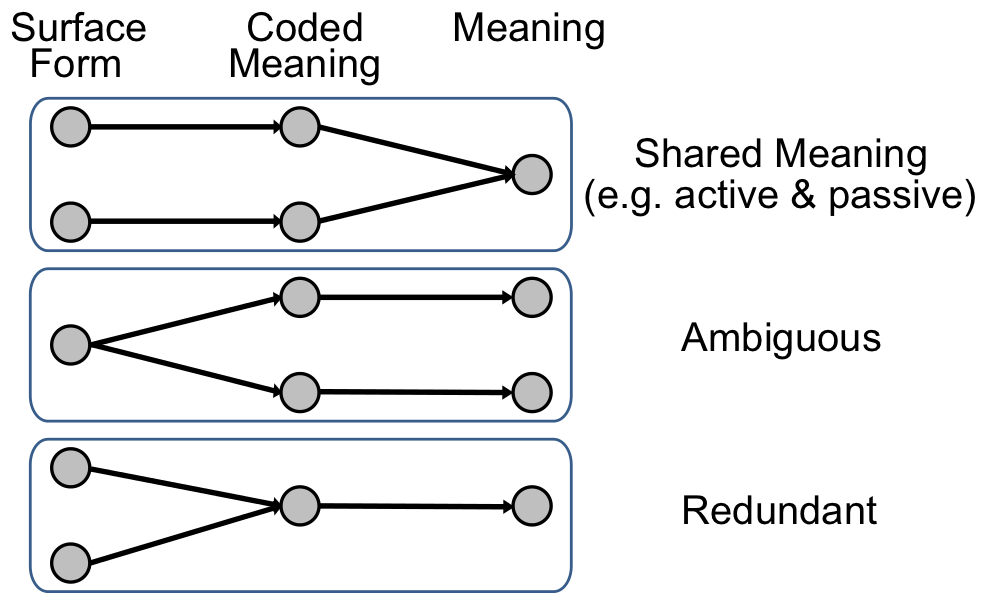
\includegraphics[width=0.5\textwidth]{meaning_relations}
\caption[Relation between sentence surface form and meanings.] {\textbf{Relation between surface form and meanings: } {\small Sentence structure to meaning mapping exist in three categories. An active and passive sentence like ``John chased the dog" and ``The dog was chased by John" have the different surface form but share the same meaning, i.e., chased(John, dog). Also, the coded meaning of both the sentences are different, i.e., SW3 (``dog") in the active form is the `Object' whereas in passive form SW3 (``John") it is an `Agent'. Ambiguous sentences have the same surface form, but different meaning and coded meaning whereas the redundant sentences have the different surface form but the coded meaning and sentence meaning. Figure adapted from \cite{xavier:2013:RT}.}}
\label{fig:meaning_realtions}
\end{figure}

\paragraph{Example-1: Ambiguous Sentences}

\begin{enumerate}[noitemsep]
\item take (SW-1) the blue (SW-2) box (SW-3) \label{eg-1:sent-1}
\item take (SW-1) the left (SW-2) box (SW-3) \label{eg-1:sent-2}
\item throw(SW-1) the green(SW-2) box(SW-3)  \label{eg-1:sent-3} 
\end{enumerate}

All the three sentences have the same surface form when transformed to abstract form by replacing the semantic words with 'SW' token, i.e., SW the SW the SW SW.

\paragraph{Training $\theta$RARes model with sentence \ref{eg-1:sent-1}:} In sentence \ref{eg-1:sent-1} there are three semantic words namely SW-1: take, SW-2: blue, SW-3: box. During the training, the sentence is input to the model from left to right, word by word, at each time step. The teacher output (semantic roles) of each semantic word is also teacher-forced as described below where, A: Action, O: Object, C: Color, I: Indicator. During the training ESN learns that the second semantic word represents a \textit{`Color'}.

\begin{table}[H]
\centering
\begin{minipage}{1.5in}
\begin{tabular}{|c|c|c|c|}
\hline
\multicolumn{4}{|c|}{\textbf{SW-1}}   \\ \hline
\textit{\textbf{A}}    & O & C & I     \\ \hline
\textit{\textbf{take}} &   &   &          \\  \hline
\end{tabular}
\end{minipage}
\begin{minipage}{1.5in}
\begin{tabular}{|c|c|c|c|}
\hline
\multicolumn{4}{|c|}{\textbf{SW-2}}                    \\ \hline
A    & O & \textit{\textbf{C}}    & I  \\ \hline
    &   & \textit{\textbf{blue}} &     \\ \hline
\end{tabular}
\end{minipage}
\begin{minipage}{1.5in}
\begin{tabular}{|c|c|c|c|}
\hline
\multicolumn{4}{|c|}{\textbf{SW-3}}                                  \\ \hline
A    & \textit{\textbf{O}}   & C    & I \\ \hline
     & \textit{\textbf{box}} &      &   \\ \hline
\end{tabular}
\end{minipage}
\end{table}

\paragraph{Training $\theta$RARes model with sentence \ref{eg-1:sent-2}:} In the sentence \ref{eg-1:sent-2}, we have three semantic words; SW-1: take, SW-2: left, SW-3: ball. Notice that only the second semantic word (SW-2) in both the sentences (\ref{eg-1:sent-1} and \ref{eg-1:sent-2}) different. Now suppose we train this sentence with a teacher output as follows where the symbols `A', `O', `C' and `I' have the same meaning as described above.

\begin{table}[H]
\centering
\begin{minipage}{1.5in}
\begin{tabular}{|c|c|c|c|}
\hline
\multicolumn{4}{|c|}{\textbf{SW-1}}   \\ \hline
\textit{\textbf{A}}    & O & C & I \\ \hline
\textit{\textbf{take}} &   &   &  \\  \hline
\end{tabular}
\end{minipage}
\begin{minipage}{1.5in}
\begin{tabular}{|c|c|c|c|}
\hline
\multicolumn{4}{|c|}{\textbf{SW-2}}                    \\ \hline
A       & O & C    & \textit{\textbf{I}} \\ \hline
 &   &  & \textit{\textbf{left}} \\ \hline
\end{tabular}
\end{minipage}
\begin{minipage}{1.5in}
\begin{tabular}{|c|c|c|c|}
\hline
\multicolumn{4}{|c|}{\textbf{SW-3}}                                  \\ \hline
A                  & \textit{\textbf{O}}   & C                  & I \\ \hline
 & \textit{\textbf{box}} & \textit{\textbf{}} &   \\ \hline
\end{tabular}
\end{minipage}
\end{table}

As both the sentences used for training have the same surface form, the ESN learning from the sentence \ref{eg-1:sent-1} may get disrupted after training with sentence \ref{eg-1:sent-2}. This is because, the second semantic word (SW-2) in the sentence \ref{eg-1:sent-2} is trained to be an \textit{`Indicator'} whereas it was trained for role \textit{`Color'} in the sentence \ref{eg-1:sent-1}. Such kind of ambiguous sentences having the same surface form but different coded meaning (roles assignment) and actual meaning, drops the learning ability of the model. We believe that this problem is mainly because each input word is treated as a discrete atomic symbol, which does not carry any semantic information about the input word \cite{w2v:tensor_flow}.

\paragraph{Testing $\theta$RARes model with sentence \ref{eg-1:sent-3}:} Now, when sentence \ref{eg-1:sent-3} is used for testing, the network may suggest two pseudo probabilities for the second semantic word, \textit{green}, i.e., being an \textit{`Indicator'} and a \textit{`Color'} as shown below. It becomes difficult for the model to resolve this ambiguity and assign the appropriate role. Although, the word \textit{green} in the test sentence \ref{eg-1:sent-3} and the word \textit{blue} in the training sentence \ref{eg-1:sent-1} are semantically related i.e., both are colors. The model cannot utilize this information as the words are input to the model in localist fashion. Thus by transforming a sentence to abstract grammatical form and using localist vector representation, the model is deprived of the semantic information carried out by a word in a language \cite{w2v:tensor_flow}.

\begin{table}[H]
\centering
\begin{minipage}{1.5in}
\begin{tabular}{|c|c|c|c|}
\hline
\multicolumn{4}{|c|}{\textbf{SW-2}}  \\ \hline
A    & O & \textit{\textbf{C(0.5)}}   & \textit{\textbf{I(0.5)}} \\ \hline
    &   & \textit{\textbf{green}}       & \textit{\textbf{green}} \\ \hline
\end{tabular}
\end{minipage}
\end{table}

\noindent Similarly, the following three sentences also have the same surface form, i.e., The SW is SW to SW.

\begin{enumerate}[noitemsep,label=(\roman*)]
\item The chicken (SW-1) is cooked (SW-2) to eat (SW-3) \label{eg-1:sent-i}
\item The ball (SW-1) is given (SW-2) to John (SW-3) \label{eg-1:sent-ii}
\item The book (SW-1) is taken (SW-2) to John (SW-3) \label{eg-1:sent-iii}
\end{enumerate}

Clearly, we can see that the third semantic word (SW-3) is a \textit{`Predicate'} in sentence \ref{eg-1:sent-i} and \textit{`Noun'} in sentence \ref{eg-1:sent-ii}. Thus, if the network is trained on sentences \ref{eg-1:sent-i} and \ref{eg-1:sent-ii} and tested on sentence \ref{eg-1:sent-iii} the network may not be able to resolve the ambiguity for semantic word SW-3, which possibly leads to wrong labelling of this word.

\paragraph{Example-2: Ambiguous and Polysemous Sentences}

\begin{enumerate}[noitemsep]
\item John (SW-1) books (SW-2) the ticket (SW-3) to London (SW-4) \label{eg-2:sent-1}
\item John (SW-1) read (SW-2) the books (SW-3) to learn (SW-4) \label{eg-2:sent-2}
\end{enumerate}

Both the above sentences share the same surface form, i.e., SW SW the SW to SW.

\paragraph{Training $\theta$RARes model on sentence \ref{eg-2:sent-1}:} When using the first sentence for training, the model learns that the fourth semantic word, \textit{London}, is a \textit{`Location'}.

\paragraph{Testing $\theta$RARes model on sentence \ref{eg-2:sent-2}:} While testing the model on the second sentence, the fourth semantic word, \textit{learn}, will be assigned the role \textit{`Location'} (as network was only trained for this) whereas it is actually an \textit{`Action'}. The reason for this mislabelling lies in the approach used to train the $\theta$RARes model. Replacing the semantic words with ``SW'' token and treating each word in the sentence as a unique identifier, removes the semantic and syntactic information carried out by a word in a language \cite{w2v:tensor_flow}. Hence, the model could not exploit the semantic information carried by a word while learning the mapping between a word and the corresponding role.

\paragraph{Issue with Polysemous words:} In the first sentence, the second semantic word \textit{books} is a \textit{`Predicate'} and describe an action of making a reservation. Whereas the same word \textit{books} in the second sentence is an \textit{`Object'}, and represents a book which we read. Although both words are same, they represent different meanings depending on the context. These kinds of words with various meaning are also known as \textit{Polysemous words}. Semantic ambiguities because of polysemous words are hard to resolve with localist vector representation where each word is treated as a unique identifier. To resolve such kind of semantic ambiguities, distributed embedding of words can be useful as they are learned using the context words and carries semantic and syntactic information about the words (e.g. Word2Vec word vectors) \cite{w2v:mikolov_2013_distributed, w2v:mikolov_2013_efficient}.

\section{Research Hypothesis}

Transformation of a sentence to its abstract grammatical form and using the localist word vectors as an input to the $\theta$RARes model has produced the promising results for the TRA task \cite{xavier:2013:RT, tra:xavier_wermter:2014, tra:xavier_hri}. However, the behavior of the model with the distributed word embeddings was left unexplored. Therefore, inspired by the limitations of $\theta$RARes model described above, this research work hypothesizes that using the distributed word embeddings (e.g. Word2Vec word embeddings) could improve the performance of the model for the TRA task. The rationale behind using distributed word embeddings to represent the words is the fact that they capture and encode semantic and syntactic information carried out by words \cite{w2v:mikolov_2013_distributed, w2v:regularities_in_word_representations}. Another advantage of using distributed word vectors is that the semantically related words remain close in the neighborhood within a word embedding space (see fig. \ref{fig:sem_rel}) \cite{w2v:mikolov_2013_distributed}. This clustering of semantically related words is however not possible when the words are represented using localist word vectors. Therefore, the use of distributed word embeddings could allow the $\theta$RARes model to learn these dynamics and avoid the disruption caused by semantically unrelated words (as explained in Example-1) in the sentences with the same grammatical constructions.

Consider using distributed embeddings of words for both the sentences in Example-2. The distributed embedding of the word, \textit{London} (sentence 1, Example-2), encodes that it represents a \textit{`Location'} along with several other semantic information. Similarly, the distributed vector representation of the word, \textit{learn} (sentence 2, Example-2), also encodes that it is a \textit{`Predicate'} along with other semantic information \cite{w2v:mikolov_2013_efficient}. When these distributed embeddings are used as an input to train the model, the learning of the model may not get disrupted by the sentences having the same surface form, but different semantic words. Hence, the roles could be assigned to the words more accurately although the sentences have the same surface form.